\def\tutdate{08.02.2018}

\documentclass{beamer}
\usepackage{../templates/beamerthemekit}
%\usepackage{enumitem}

\usepackage[utf8]{inputenc}
\usepackage[T1]{fontenc}
\usepackage[ngerman]{babel}
\usepackage{listings}
\usepackage{hyperref}
\usepackage{graphicx}

\usepackage{amsmath}
\usepackage{amsthm}
\usepackage{amssymb}
\usepackage{polynom}

%\usepackage{ifthen}
%\usepackage{adjustbox} % for \adjincludegraphics

%\usepackage{tikz}
\usepackage{listings}

%\usepackage[]{algorithm2e}

%\usepackage{colortbl}
\usepackage{verbatim}
%\usepackage{alltt}
%\usepackage{changes}

%\usepackage{pdfpages}
%\usepackage{tabularx}

%\usepackage{euler}


\newcommand{\markBlue}[1]{\textcolor{kit-blue100}{#1}}
\newcommand{\markGreen}[1]{\textcolor{kit-green100}{#1}}
\newcommand{\vertspace}{\vspace{.2cm}}

%\newcommand{\#}{\markBlue{#1}}

%\newcommand{\pitem}{\pause\item}
\newcommand{\p}{\pause}

% -- MATH MACROS
\newcommand{\thistheoremname}{}
\newcommand{\G}{\mathbb{Z}}
\newcommand{\B}{\mathbb{B}}
\newcommand{\R}{\mathbb{R}}
\newcommand{\N}{\mathbb{N}}
\newcommand{\Q}{\mathbb{Q}}
\newcommand{\C}{\mathbb{C}}
\newcommand{\Z}{\mathbb{Z}}
\newcommand{\F}{\mathbb{F}}
\newcommand{\mi}{\mathrm{i}}
\renewcommand{\epsilon}{\varepsilon}
\newcommand{\okalk}{\mathscr{O}}


\newenvironment<>{taskblock}[1]{%
	\setbeamercolor{block title}{fg=kit-orange15,bg=kit-orange100}
	\setbeamercolor{block body}{fg=black,bg=kit-orange30}%
	\begin{block}#2{#1}}{\end{block}}

\setbeamertemplate{enumerate items}[default]

% Aussagenlogik Symbole
\newcommand{\W}{w}
\renewcommand{\F}{f}

% Kodierung
\newcommand{\frepr}{\textbf{repr}}
\newcommand{\fRepr}{\textbf{Repr}}
\newcommand{\fZkpl}{\textbf{Zkpl}}
\newcommand{\fbin}{\textbf{bin}}
\newcommand{\fdiv}{\textbf{ div }}
\newcommand{\fmod}{\textbf{ mod }}

% Speicherabbild
\newenvironment{memory}{\begin{tabular}{r | l}Adresse&Wert\\\hline\hline}{\end{tabular}}
\newcommand{\memrow}[2]{#1 & #2 \\\hline}

% Praedikatenlogik
\newcommand{\objequiv}{\stackrel{\cdot}{=}}
\newcommand{\pval}{val_{D,I,\beta}}

% Neue Befehle
\newcommand{\ip}{\pause} % inline pause, für mitten im satz
\newcommand{\pitem}{\pause\item} % für aufzählungen
\newcommand{\bp}{\pause} % block pause, für zwischen blöcken
\title[Grundbegriffe der Informatik]{ICPC\\Gruppe 2}
\date{\tutdate}
\subtitle{\tutTitle}
\author{Elias Schaut, Dennis Kobert, Niklas Kniep, Lam Vo, Ilia Bozhinov}

\institute{}

\titleimage{bg}
%\titleimage{bg-advent}

%
\ifthenelse{\equal{\compiletype}{livebeamer}}
	{
		\def\livebeamermode{1}
	}{}

\ifthenelse{\equal{\compiletype}{print}}
	{
		\def\printmode{1}
	}{}

\setbeamercovered{invisible}

%\usepackage[citestyle=authoryear,bibstyle=numeric,hyperref,backend=biber]{biblatex}
%\addbibresource{templates/example.bib}
%\bibhang1em

	
\def\tutTitle{Turingmaschinen}
\begin{document}

\selectlanguage{ngerman}

%title page
\begin{frame}
	\titlepage
\end{frame}

\section{Turingmaschinen}

\begin{frame}{Turingmaschinen}
	Was sind Turingmaschinen?
	
	\begin{itemize}
		\pitem Sehr mächtige Erweiterung Automat
		\begin{itemize}
			\pitem Was heißt mächtig?
			\pitem Turingmaschinen können eine große Vielfalt von Problemen lösen, einschließlich vieler in GBI besprochener Probleme
		\end{itemize}
		\pitem Gesteuert durch einen endlichen Automaten\ip, aber mit einem \markBlue{unendlichen Arbeitsband} zum Zwischenspeichern von Informationen
		\pitem Besitzen einen Kopf um auf dem Band zu lesen und zu schreiben
		\pitem Turingmaschinen sind sozusagen genauso mächtig wie Computer
		\begin{itemize}
			\pitem können also benutzt werden, um für Probleme zu entscheiden, \markGreen{ob sie gelöst werden können oder nicht}
		\end{itemize}
	\end{itemize}
\end{frame}

\begin{frame}{Definition von Turingmaschinen}
	\begin{block}{Definition von Turingmaschinen}
		Eine Turingmaschine $T = (Z, z_0, X, f, g, m)$ besteht aus:
		\begin{itemize}
			\pitem $Z$ Zustandsmenge
			\pitem $z_0 \in Z$ Startzustand
			\pitem $X$ Bandalphabet
			\pitem $\Box$ Blanksymbol (sozusagen Markierung für Leerzeichen)
			\pitem $f: Z \times X \rightarrow Z$ partielle Zustandsübergangsfunktion
			\pitem $g: Z \times X \rightarrow X$ partielle Ausgabefunktion
			\pitem $m: Z \times X \rightarrow \{L, N, R\}$ partielle Bewegungsfunktion
		\end{itemize}
	\end{block}

	Anmerkung: partielle Funktionen sind \markGreen{nicht linkstotal}, also manche Elemente des Definitionsbereichs werden nicht abgebildet.
\end{frame}

\begin{frame}{Beispiel einer Turingmaschine}
	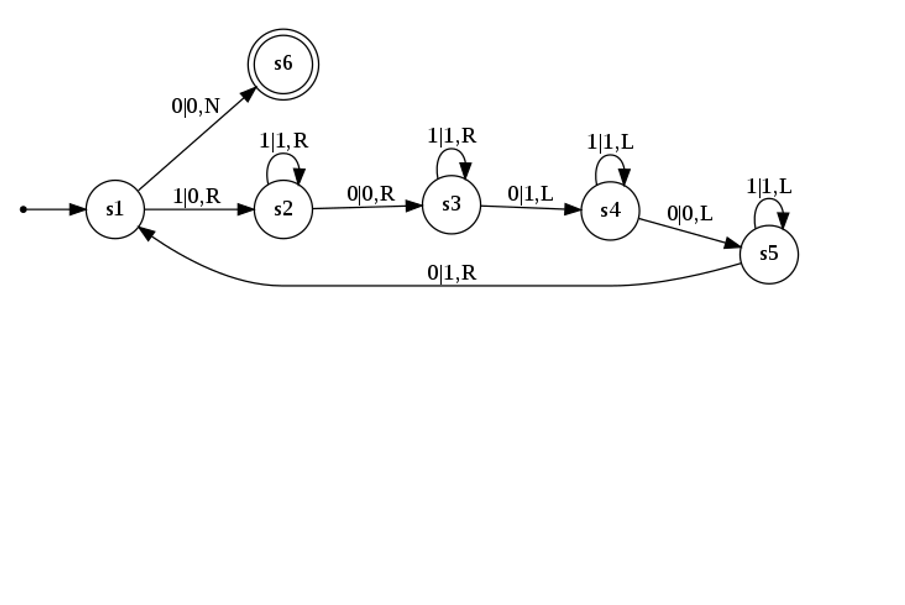
\includegraphics[scale=0.5]{images/turingexample_withoutannotations.png}
\end{frame}

\begin{frame}{Beispiel einer Turingmaschine}
	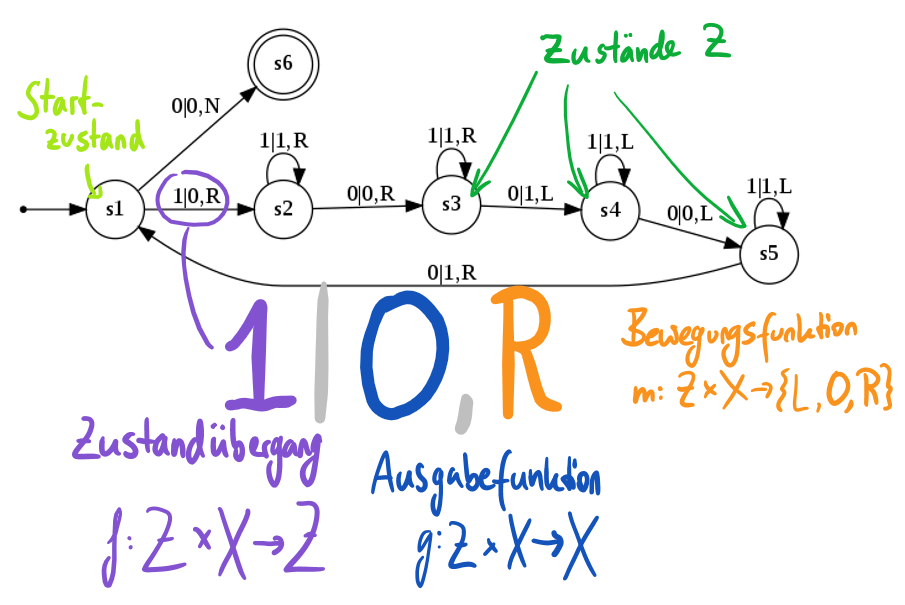
\includegraphics[scale=0.5]{images/turingexample_withannotations.png}
\end{frame}

\begin{frame}{Funktionen von Turingmaschinen}
	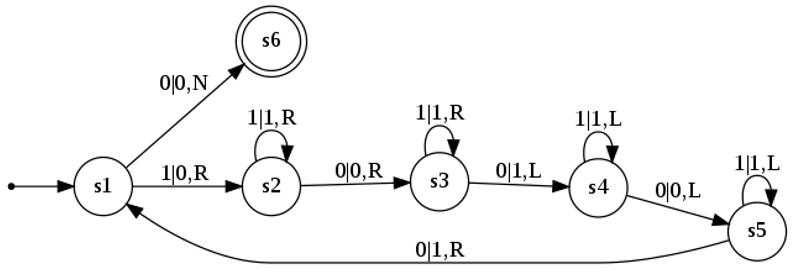
\includegraphics[scale=0.4]{images/turingexample_smallspacing.png}
	
	Wie sehen die konkreten Abbildungsvorschriften der linken vier Pfeile aus?
	
	\begin{columns}
		\begin{column}{0.3\textwidth}
			
			\vspace{.2cm}
			
			% vielleicht an die tafel schreiben was die funktionen vom namen her machen (f: zustandsübergang), hat so nicht mehr auf die folie gepasst
			\begin{itemize}
				\item $f: Z \times X \rightarrow Z$
				\item $g: Z \times X \rightarrow X$
				\item $m: Z \times X \rightarrow \{L, N, R\}$
			\end{itemize}
		\end{column}
		
		\begin{column}{0.7\textwidth}
			\begin{tabular}{r || c | c | c}
				 & f & g & m\\\hline\hline
				 
				 %erste Zeile als Beispiel
				 $0|0,N$ & $(s1, 0) \mapsto s6$ & $(s1, 0) \mapsto 0$ & $(s1, 0) \mapsto N$ \\\hline
				 
				 \pause $1|0, R$ 
				 \pause & $(s1, 1) \mapsto s2$
				 \pause & $(s1, 1) \mapsto 0$
				 \pause & $(s1, 1) \mapsto R$ \\\hline
				 
				 \pause $1|1, R$ 
				 \pause & $(s2, 1) \mapsto s2$
				 \pause & $(s2, 1) \mapsto 1$
				 \pause & $(s2, 1) \mapsto R$ \\\hline
				 
				 \pause $0|0, R$ 
				 \pause & $(s2, 1) \mapsto s3$
				 \pause & $(s2, 1) \mapsto 0$
				 \pause & $(s2, 1) \mapsto R$ \\\hline
				
			\end{tabular}
		\end{column}
	\end{columns}

\end{frame}


\begin{frame}{Das Band einer Turingmaschine}
	\begin{itemize}
		\pitem Unendliche Anreihung von Zeichen, die nach links und rechts unbegrenzt weiter geht
		
		\p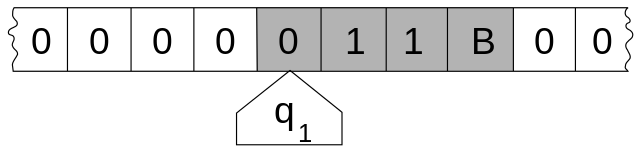
\includegraphics[scale=0.3]{images/turing_band.png}
		
		\pitem Die Turingmaschine hat einen Kopf, mit dem sie das aktuelle Zeichen lesen oder überschreiben kann, oder kann ihn nach links oder rechts bewegen.
		
		\pitem Das Band einer Turingmaschine wird benutzt als...
		\begin{itemize}
			\pitem Erhalten der Eingabe: \ip Bevor die Turingmaschine startet, steht das Eingabewort auf dem Band, der Kopf steht auf dem ersten Zeichen der Eingabe.
			\pitem Rückgabe der Ausgabe: \ip Nach Beenden steht auf dem Band die Ausgabe (und der Kopf irgendwo).
			\pitem Zwischenspeicher: \ip Die Turingmaschine kann überall Informationen zwischenspeichern, diese müssen von der TM am Ende aber gelöscht werden.
		\end{itemize}
	\end{itemize}
\end{frame}
	
% Am besten erst mal die aufgaben zusammen durchrechnen
\begin{frame}{Beispielabarbeitungen}
	\begin{columns}
		\begin{column}{0.5\textwidth}
			\begin{taskblock}{Gemeinsame Übung}
				Arbeite folgende Wörter mit der Turingmaschine ab:
				\begin{itemize}
					\item $0$
					\item $1$
					\item $11$
					\item $111$
				\end{itemize}
				Was macht die Turingmaschine?
			\end{taskblock}
		\end{column}
	
		\begin{column}{0.5\textwidth}
			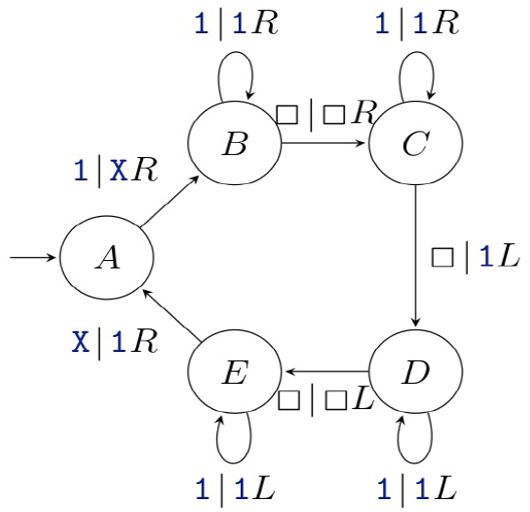
\includegraphics[scale=0.4]{images/turingmaschine_1k.png}
		\end{column}
	\end{columns}

	\pause
	
	Die Turingmaschine macht aus $1^k$ die Ausgabe $1^k \Box 1^k$.
\end{frame}

\begin{frame}{Halten von Turingmaschinen}
	
	\p
	
	\begin{block}{Halten einer Turingmaschine}
		Wenn eine Turingmaschine in einem Zustand ist, für den das nächste Eingabezeichen durch die Übergangsfunktion $f$ nicht definiert ist, \markGreen{hält} die Maschine.
	\end{block}

	\bp

	Wann hält also eine Turingmaschine \markBlue{nicht}?
	
	\bp
	
	\begin{block}{Nicht-Halten einer Turingmmaschine}
		Wenn eine Turingmaschine in eine endlose Schleife gerät, so \markGreen{hält sie nicht}.
	\end{block}
\end{frame}

\begin{frame}{Entscheidbarkeit}
	\ip
	
	\begin{block}{Durch Turingmaschine akzeptierte Sprache}
		Eine Turingmaschine \markBlue{akzeptiert} eine formale Sprache $L$, wenn sie für jedes Wort $w \in L$ in einem akzeptierenden Zustand hält.
	\end{block}

	\bp

	\begin{block}{Entscheidbare Sprache}
		Eine formale Sprache $L$ heißt \markBlue{entscheidbar}, wenn es eine Turingmaschine gibt, die \markGreen{immer hält} und $L$ akzeptiert.
	\end{block}

	\bp

	\begin{block}{Aufzählbare Sprache}
		Eine formale Sprache $L$ heißt \markBlue{aufzählbar}, wenn es eine Turingmaschine gibt, die $L$ akzeptiert.
	\end{block}
\end{frame}

\begin{frame}{Vom endlichen Akzeptor zur Turingmaschine}
	\begin{taskblock}{Akzeptieren von Turingmaschinen}
		Wie kann man aus dem gegebenen endlichen Akzeptor eine Turingmaschine machen, die dieselbe Sprache akzeptiert?
	\end{taskblock}

	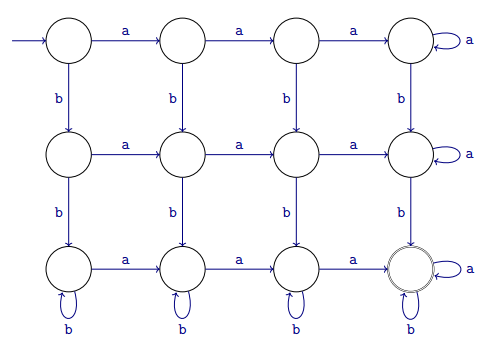
\includegraphics[scale=0.5]{images/AufgAkzeptor2.png}
\end{frame}

\begin{frame}{Lösung}
	Einfach gesagt: mache aus jedem Übergang $a$ einen Turingmaschinen-Übergang der Art $a|a,R$, also bei jedem Zeichen mache den Zustandsübergang, überschreibe aber das Zeichen nicht und gehe zum nächsten Zeichen.
	
	\vspace{.2cm}
	\bp
	
	Formaler ausgedrückt? \pause 
	\begin{itemize}
		\item Für allgemeinen endlichen Akzeptor $(Z, z_0, X, f, Y, h)$, definiere eine Turingmaschine $T := (Z, z_0, X \cup Y, f, g, h)$, also $Z, z_0, f$ gleich und mit Bandalphabet $=$ Eingabealphabet $\cup$ Ausgabealphabet
		\item $g(z, x) := x \quad \forall (z,x)$ in $f$ definiert
		\item $m(z, x) := R \quad \forall (z,y)$ in $f$ definiert		
	\end{itemize}

	\bp
	
	Jeder endliche Akzeptor kann so zu einer Turingmaschine umgeformt werden, die dieselbe Sprache akzeptiert.
\end{frame}

\begin{frame}{Über endliche Akzeptoren hinaus}
	Sei $L$ die Sprache von Palindromen über $\{a,b\}$ ($L = \{aabaa, bbababb, aa, \epsilon\}$). 
	
	\begin{itemize}
		\pitem Ist die Sprache regulär, also gibt es einen endlichen Akzeptor, der diese akzeptiert? \pause Nein.
		\pitem Ist die Sprache entscheidbar, also gibt es eine stets haltende Turingmaschine, die $L$ akzeptiert?
	\end{itemize}
\end{frame}

\begin{frame}{Palindromerkennung mit Turingmaschinen}
	Ja, nämlich: 
		
	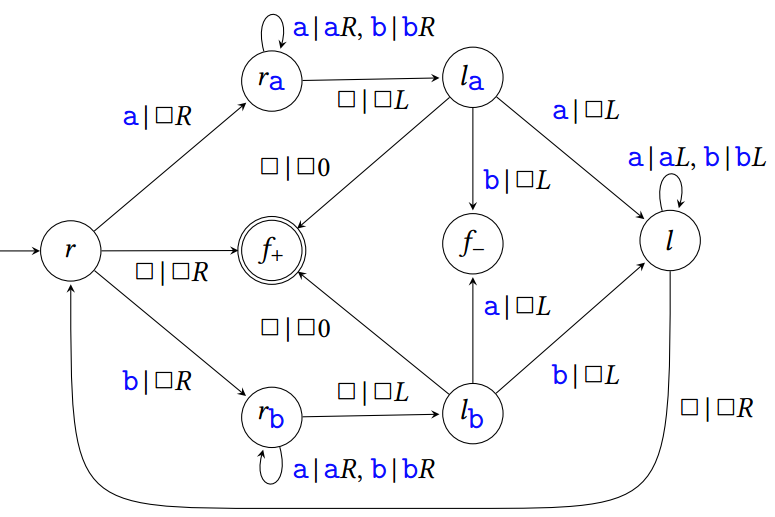
\includegraphics[scale=0.5]{images/turingmaschine_palindrome.png}	
\end{frame}

\begin{frame}{Turingmaschinen Entwurfsaufgabe}
	
	\begin{columns}
		\begin{column}{0.65\textwidth}
			\begin{taskblock}{Turingmaschine Entwurf}
				Entwerfe eine Turingmaschine, die...
				\begin{itemize}
					\item als Eingabe eine Binärzahl auf dem Band erhält
					\item als Ausgabe diese Zahl restlos durch zwei teilt und auf dem Band stehen lässt
				\end{itemize}
			\end{taskblock}
		\end{column}
		
		\begin{column}{0.45\textwidth}
			\pause
			
			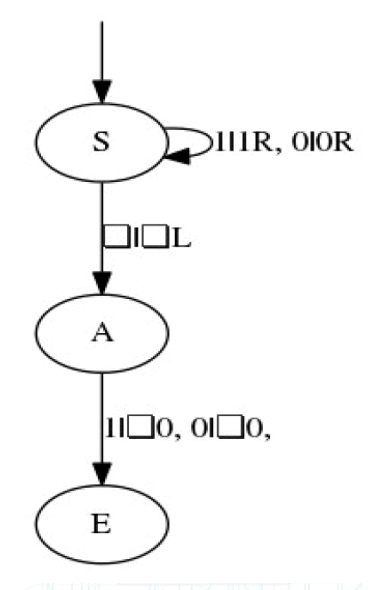
\includegraphics[scale=0.45]{images/turingmaschine_div.png}
		\end{column}
	\end{columns}

\end{frame}

\begin{frame}{Turingmaschinen Entwurfsaufgabe}
	
	\begin{columns}
		\begin{column}{0.65\textwidth}
			\begin{taskblock}{Turingmaschine Entwurf}
				Entwerfe eine Turingmaschine, die...
				\begin{itemize}
					\item als Eingabe eine Binärzahl auf dem Band erhält
					\item als Ausgabe diese Zahl um eins erhöht auf dem Band stehen lässt
					\item den Kopf der Turingmaschine auf dem ersten Zeichen der Ausgabe stehen hat.
				\end{itemize}
			\end{taskblock}
		\end{column}
		
		\begin{column}{0.45\textwidth}
			\pause
			
			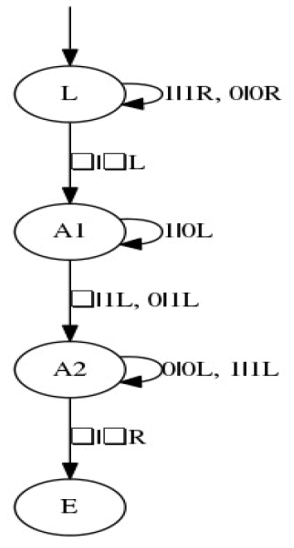
\includegraphics[scale=0.5]{images/turingmaschine_plusone.png}
		\end{column}
	\end{columns}
	
\end{frame}

\begin{frame}{Turingmaschine Entwurfsaufgabe}
	
	\begin{taskblock}{Turingmaschine Entwurf}
		Entwerfe eine Turingmaschine, die die Sprache $\{a^kb^k : k \in \N_0 \}$ erkennt.
	\end{taskblock}
	\pause
	
	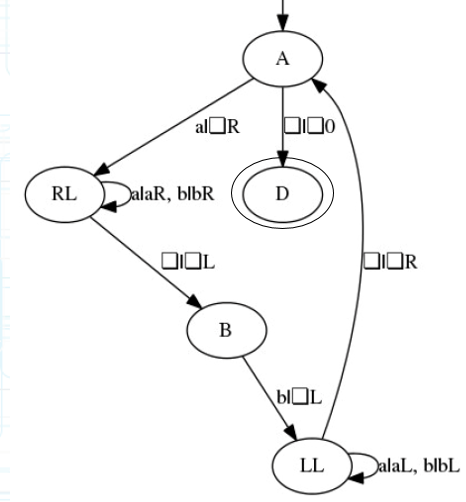
\includegraphics[scale=0.4]{images/turingmaschine_aabb.png}
	
\end{frame}

\begin{frame}{Konfiguration von Turingmaschinen}
	Angenommen, man kennt eine Turingmaschine, hat mit der Abarbeitung eines Wortes angefangen, will aber pausieren, um später weiterzumachen...
	
	\vspace{.2cm}
	
	Was muss man sich alles merken, um später weiter zu machen?
	
	\begin{itemize}
		\pitem Derzeitiger Zustand, in dem die Turingmaschine steht
		\pitem Inhalt des Bandes
	\end{itemize}

	\bp
	\vspace{.2cm}
	
	\begin{block}{Konfiguration von Turingmaschinen}
		Wenn während dem Arbeiten einer Turingmaschine auf dem Band das Wort $w_1 a w_2$ mit $w_1, w_2 \in X^*, a \in X$ steht\ip, der Kopf der Turingmaschine auf das Zeichen $a$ zeigt \ip und die Turingmaschine im Zustand $z$ ist\ip, so schreibt man die \markBlue{Konfiguration der Turingmaschine} als $\Box w_1 (z) a w_2 \Box $.
	\end{block}
\end{frame}

\begin{frame}{Konfiguration von Turingmaschinen}
	Beispiel:
	
	\vspace{.2cm}
	
	\begin{align*}
	\Box\Box\Box\Box\Box\Box\Box\Box abcbabb&\markBlue{d}aabc \Box\Box\Box\Box\Box \\
	&\uparrow \\
	&KOPF
	\end{align*}
	
	\bp
	...sei das Band der Turingmaschine während Abarbeitung der Eingabe, dazu steht sie im Zustand $z_4$.
	
	\vspace{.2cm}
	
	\bp
	Dann sieht sieht die Konfiguration der Turingmaschine so aus: \ip $\Box abcbabb (z_4) daabc \Box$
\end{frame}

\begin{frame}{Dokumentation einer Abarbeitung mit Konfigurationen}
	
	\begin{taskblock}{Aufgabe zu Konfigurationen}
		Gebe alle Konfigurationen der Turingmaschine bei Abarbeitung des Wortes $11$ an.
	\end{taskblock}

	\begin{columns}
		\begin{column}{0.25\textwidth}
			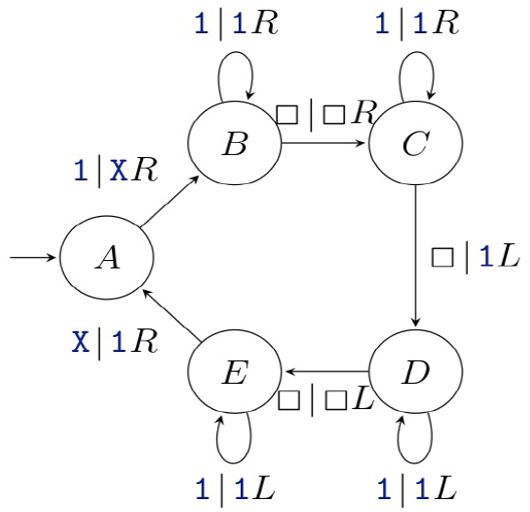
\includegraphics[scale=0.3]{images/turingmaschine_1k.png}
		\end{column}
		
		\begin{column}{0.4\textwidth}
			\begin{description}
				\pause\item[] $\Box (A)11 \Box$
				\pause\item[$\rightarrow$] $\Box X(B)1 \Box$
				\pause\item[$\rightarrow$] $\Box X1(B) \Box$
				\pause\item[$\rightarrow$] $\Box X1 \Box (C) \Box$
				\pause\item[$\rightarrow$] $\Box X1 (D) \Box 1\Box$
				\pause\item[$\rightarrow$] $\Box X (E) 1 \Box 1\Box$
				\pause\item[$\rightarrow$] $\Box (E) X 1 \Box 1\Box$
				\pause\item[$\rightarrow$] $\Box 1 (A) 1 \Box 1\Box$
			\end{description}
		\end{column}
	
		\begin{column}{0.4\textwidth}
			\begin{description}
				\pause\item[$\rightarrow$] $\Box 1 X (B) \Box 1\Box$
				\pause\item[$\rightarrow$] $\Box 1 X \Box (C) 1\Box$
				\pause\item[$\rightarrow$] $\Box 1 X \Box 1 (C)\Box$
				\pause\item[$\rightarrow$] $\Box 1 X \Box (D) 1 1\Box$
				\pause\item[$\rightarrow$] $\Box 1 X (D) \Box 1 1\Box$
				\pause\item[$\rightarrow$] $\Box 1 (E) X \Box 1 1\Box$
				\pause\item[$\rightarrow$] $\Box 1 1 (A) \Box 1 1\Box$
			\end{description}
		\end{column}
	\end{columns}
\end{frame}

\begin{frame}{Halteproblem}
	\markBlue{Halteproblem}: Für einen gegebenen Algorithmus, gelingt dieser bei seiner Abarbeitung zu einem Ende und hält?
	
	\begin{itemize}
		\pitem Algorithmen können durch Turingmaschinen durchgeführt werden
		\pitem Turingmaschinen können durch sogenannte universelle Turingmaschinen simuliert werden
		\begin{itemize}
			\pitem Wenn eine Turingmaschine $T$ kodiert ist mit dem Wort $w$, dann ist $T_w: X \rightarrow X$ eine Funktion, die Eingaben auf die Ausgabe der Turingmaschine $T$ mappt.
			\pitem Also mit $X = \{1,0\}$ gibt z.B. $T_w(100101) = 001$ genau dann zurück, wenn, sofern man $100101$ als Eingabe an die Turingmaschine mit der Kodierung $w$ gibt, diese hält und als Ausgabe $001$ erzeugt.
		\end{itemize}
	\end{itemize}

	\bp
	
	Dann lässt sich das Halteproblem auch als Sprache formulieren:
	
	\vspace{.2cm}
	
	$\quad H = \{w \in A^* : w \text{ ist eine TM-Codierung und } T_w(w) \text{ hält.}\}$
	
	bzw. als allgemeinerer Fall:
	
	$\quad \hat{H} = \{(w,x) \in A^* \times A^* : w \text{ ist eine TM-Codierung und } T_w(x) \text{ hält.}\}$
\end{frame}

\begin{frame}{Halteproblem}
	Das Halteproblem ist unentscheidbar\ip, dh. es gibt keine Turingmaschine, die $H$ entscheidet.
\end{frame}

\begin{frame}{Busy Beaver}
	\markBlue{Busy Beaver TM} ist eine Turingmaschine mit $n$ Zuständen, die möglichst viele Einsen auf das Band schreibt \markBlue{und hält}.
	
	\begin{itemize}
		\pitem Also nicht einfach ewig Einsen aufschreibt und nie aufhört.
	\end{itemize}
	
	\bp
	
	\markBlue{Busy Beaver Problem}: Für eine gegebene Turingmaschine mit $n$ Zuständen, die Einsen aufschreibt und hält: Schreibt sie auch maximal viele Einsen auf?
	
	\bp
	\vspace{.2cm}
	
	Das Busy Beaver Problem ist nicht entscheidbar, bzw. die Busy Beaver Funktion $bb(n)$, die definiert, wieviele einsen von einer Busy Beaver TM maximal geschrieben werden können, ist nicht berechenbar.
	
	\bp
	
	\vspace{.2cm}
	
	Beispielwerte von $bb$: $bb(1) = 1\ip, bb(2) = 4\ip, bb(5) \geq 4098\ip, bb(6) > 10^{18276}$.
\end{frame}

\begin{frame}{Busy Beaver für $n = 3$}
	% 3 zustände und ein haltezustand	
	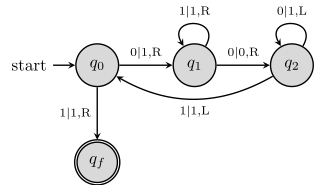
\includegraphics[scale=0.8]{images/turingmaschine_bb.png}	
\end{frame}

\begin{frame}{Organisatorisches}
	% Noch zeigen:
	% assets/Tut14E_AufgabenverteilungBis12-13.png (jetzt aber mit prädikatenlogik und evtl mima!)
	% assets/Tut14F_Notenverteilung11-12.png 
	\begin{itemize}
		\item Alle Folien und Folienpaket jetzt online.
		\item Fragen zur Klausur oder zur Vorbereitung?
	\end{itemize}
\end{frame}


\begin{frame}
	
\includegraphics[width=\linewidth]{../images/thatsall.png}
\end{frame}


\end{document}